\maketitle

\begin{abstract}
In the life-cycle of objects there are different phases. The phase in which an object currently is, affects how it is handled in an application; however phase shifts are typically implicit.
In this study we propose an extension to the aspect-oriented language AspectJ with a new mechanism, called \emph{instance pointcuts}, for categorizing objects according to events in their life-cycle; these events are selected with pointcut-like specifications.
The selection criteria of instance pointcuts can be refined, e.g., by restricting the scope of an existing instance pointcut; and they can be composed, e.g., by boolean operations.
We offer a means to access all objects currently selected by an instance pointcut from Java code, i.e., to be used in methods or advice bodies; and we expose the events of adding or removing an object from an instance pointcut by creating a join point that can be selected by regular pointcuts.
Our approach improves modularity by providing a fine-grained mechanism and a declarative syntax to define and maintain object categories.
\end{abstract}

% A category with the (minimum) three required fields
\category{D.3.1}{Formal Definition and Theory}[syntax, semantics]
%A category including the fourth, optional field follows...
\category{D.3.4}{Processors}[code generation]

\section{Introduction}
In object-oriented programming (OOP), objects encapsulate state and behavior; objects also have a life-cycle, which means that the same object can play different roles at different times.
Which role an object is currently playing can affect the object's own behavior or how it is handled.
Typically the shift from one life-cycle phase to another is implicitly marked by events, e.g., passing an object from one client to another.
Aspect-oriented programming (AOP) is a well-known technique for modularly implementing behavior applicable at events emitted from code that is not localized in a single type hierarchy.
But current aspect-oriented languages do not offer declarative abstractions of object sets based on other criteria then the type.
In this paper, we propose a new language mechanism for declaratively specifying life-cycle phases and for categorizing a set of objects which are currently in a specific phase. This declarativity allows us to perform compile-time checks like warning about sets that will always be empty. 
%\textbf{Do we discuss checks?}

As an example of different relevant phases in the life-cycle of objects, consider an online store application with ``customer'' objects representing the purchasers and ``item'' objects representing the products they add to their ``shopping bags''. We want to add discount policies for products that are treated by the customers in specific ways: For instance, a discount may apply for items that have been added to the shopping bag during the ``happy hour''. Thus, when calculating the price at check-out, we need to know which objects have been shopped within this hour.
Categorizing objects according to criteria not directly supported by the programming language, such as the class they were initialized in, the method they are passed to as an argument, or (as in the example) the time at which they are passed to a method, requires invasively inserting bookkeeping code.

Aspect-oriented programming can be applied to separate this bookkeeping code from the business logic of the program. But in AOP, \emph{pointcuts} select sets of so-called \emph{join points} which are points in time during the execution of the program. Current aspect-oriented languages do not support a \emph{declarative specification} of the objects belonging to a life-cycle phases; instead an \emph{imperative implementation}, always following the same pattern, is required for collecting those objects.
A consequence of such an imperative solution, besides all the negative effects of hand-writing boilerplate code, is that automatic reasoning becomes practically impossible. 
%\textbf{checking}

To offer better support for processing objects according to their life-cycle phase, we propose to extend aspect-oriented programming languages.
For this matter, we propose a new mechanism, called \emph{instance pointcuts}, to select sets of objects based on the execution history.
An instance pointcut definition consists of three parts: an identifier, a type which is the upper bound for all objects in the selected set, and a specification of relevant objects.
The specification utilizes \emph{pointcut expressions} to select events that define the begin and end of life-cycle phases and to expose the object. At these events, an object is added or removed from the set representing the instance pointcut.

New instance pointcuts can be derived from existing ones. Firstly, a new instance pointcut can be derived from another one by restricting the type of selected objects. 
%Secondly, a \emph{subset} or a \emph{super-set} of an existing instance pointcut can be declared whereby the specification of the life-cycle phase is either narrowed down or broadened. 
Secondly, instance pointcut declarations can be composed arbitrarily by means of boolean operators. In this paper we present instance pointcuts as an extension to AspectJ \cite{kiczales2001overview} and explain its semantics by explaining our compiler which transforms instance pointcuts to plain AspectJ and advanced dispatching library calls. 


\emph{TO THE REVIEWER: A version of this paper is submitted to SLE2012 conference. In case that submission gets accepted, this paper will be withdrawn from AOSD2013. There is new material in this paper, which is not present in the SLE2012 submission. This paper includes a section on compilation, which presents a complete implementation whereas the SLE paper only presents a possible compilation option which is also different from the compilation method presented here. We have also dropped some part of the instance pointcut syntax in this paper, which was found redundant after further consideration.}

\section{Motivation}
\label{sect:motivation}

Objects can be categorized by how they are used (passed as arguments to method calls, act as receiver or sender for method calls, etc.) and concerns of an application may be applicable only to objects used in a specific way.
Therefore we must be able to identify and select those objects.
We want to expose sets of objects belonging to the same category by means of a dedicated language construct such that the implementation of context-dependent concerns can explicitly refer to the category.

\begin{figure*}
\centering
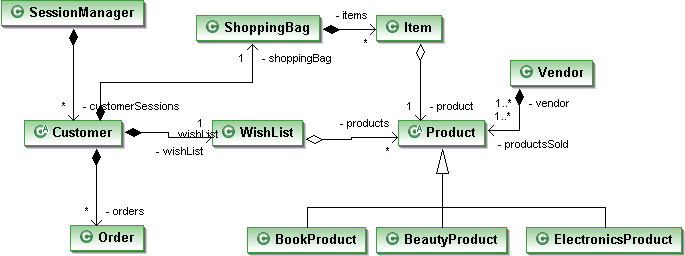
\includegraphics[width= 0.75\textwidth]{images/myonlineshop.png}%
\vspace{10pt}
\caption{A simple online shop application}%
\label{fig:shop}%
\end{figure*}

Below, we outline the architecture and design of an online store application. We use this scenario to give examples of categorizing objects according to how they are used and how to use these categories in the implementation of concerns. It must be noted that we intend to support the addition of \emph{unanticipated} concerns, i.e., the program code is not prepared to support abstractions, like specific object categories, required by the new concerns.
At the end of this section, we conclude requirements for solving the encountered challenges in these examples.

\subsection{Example Architecture}
An online shop is a sophisticated web application and objects of the same type can exist at different stages of the life-cycle. In Figure~\ref{fig:shop} the static structure of a simplified online shop is shown. When a new user logs in, \lstinline{SessionManager} creates a \lstinline{Customer} object to represent the user's session. A customer has a \lstinline{ShoppingBag} and a \lstinline{WishList}. The abstract class \lstinline{Product} is a super-type of all products in the shop and represents product data. The \lstinline{Product}'s subclasses are \lstinline{BeautyProduct}, \lstinline{BookProduct} etc. When the customer selects a product and clicks ``add to shopping bag'', a new \lstinline{Item} instance is created and added to the \lstinline{ShoppingBag} object; the \lstinline{Item} instance contains the \lstinline{Product} and quantity of that \lstinline{Product}. A customer can add/remove items from his shopping bag. When the shopping is finished the \lstinline{checkOut()} method is invoked on \lstinline{Customer}, which returns an object of type \lstinline{Order}. A \lstinline{Customer} can also add or remove \lstinline{Product}s to/from his \lstinline{WishList}; the \lstinline{WishList} holds a list of \lstinline{Products}, whereas \lstinline{ShoppingBag} holds a list of \lstinline{Item}s.

\subsection{Unanticipated Extensions}
Let's assume a new requirement for applying a happy-hour discount is introduced. The discount should be applied at check-out to \lstinline{Item}s which have been added to a customer's shopping bag between certain hours.
In order to realize this extension in an OO-approach, one needs to invasively change the system code: First we need to keep a set of items that were added to a shopping bag within the timing condition. When the user finally checks out, we have to apply the discount to the items in the set. Listing~\ref{lst:happyhour} shows that we need to insert code in multiple places to satisfy the new requirement. First a set, called \lstinline{happyItems}, is created (Line~\ref{lst:happyhour:happyitems}) in class \lstinline{ShoppingBag}, to keep track of items that are added during the happy-hour. In the \lstinline{addToShoppingBag} method the timing condition is checked, and when the condition is satisfied the created \lstinline{Item} is added to \lstinline{happyItems} (Lines~\ref{lst:happyhour:add:begin}--~\ref{lst:happyhour:add:end}).  In the \lstinline{Customer} class, more code is inserted to the \lstinline{checkOut} method to apply the discount to the items in \lstinline{happyItems} set (Line~\ref{lst:happyhour:checkout}). 

\begin{lstlisting}[float, caption={A Java implementation of happy-hour discount rule}, label={lst:happyhour}]
class ShoppingBag{
	...
	Set<Item> happyItems = createSet(); ~\label{lst:happyhour:happyitems}~
	public boolean addToShoppingBag(Product p, int amount)
	{
		Item item = ItemFactory.createItem(p,amount); ~\label{lst:happyhour:add:begin}~
		if('timing condition')
			happyItems.put(item);~\label{lst:happyhour:add:end}~
		...
	}
	public boolean removeFromShoppingBag(Item item, int amount)
	{
		...
		happyItems.remove(item);
	}
}
class Customer{
	...
	public checkOut()
	{
		ProductManager. applyHappyHourDiscount(this.shoppingBag.happyItems);~\label{lst:happyhour:checkout}~
	}
}
\end{lstlisting}

The OO-solution is scattered among \lstinline{ShoppingBag} and \lstinline{Customer} classes and tangled to multiple methods. Even for a single discount rule, the code for the discount concern and the book-keeping that comes with it creates cluttering. If we would like to apply multiple discount rules for the \emph{check-out} event, this implementation style is clearly not suitable.
An aspect-oriented implementation can offer a better solution by encapsulating the concern in an aspect. In Listing~\ref{lst:happyhouraop} the \lstinline{newItem} pointcut (Lines~\ref{lst:happyaop:newitem:b}--~\ref{lst:happyaop:newitem:e}) selects join-points where a customer adds a product to his bag: A new \lstinline{Item} is created in the \lstinline{addToShoppingBag} method. The advice is executed when \lstinline{newItem} is matched; after returning the new \lstinline{Item}, the timing condition is checked and if it holds it is added to \lstinline{happyItems}. 
%\textbf{the condition should better be checked in an if-pointcut.}

We also define the \lstinline{removeItem} pointcut (Lines~\ref{lst:happyaop:remove:b}--~\ref{lst:happyaop:remove:e}) and advise it (Lines~\ref{lst:happyaop:remadvice:b}--~\ref{lst:happyaop:remadvice:e}) to remove an item from \lstinline{happyItems} if it is removed from a shopping bag.
Finally, we define a pointcut for selecting the \lstinline{Customer.checkOut()} join-point (Lines~\ref{lst:happyaop:checkout:b}--~\ref{lst:happyaop:checkout:e}) and before the method is executed we apply the discount to items in \lstinline{happyItems}.
%An AO implementation, although offers a non-invasive solution, also suffers from boilerplate code written for book-keeping. 

\begin{lstlisting}[float=h, caption={An Aspectj implementation of happy-hour discount rule}, label={lst:happyhouraop}]
Set<Item> happyItems = createSet();
pointcut newItem(Item item): ~\label{lst:happyaop:newitem:b}~
	call(* ItemFactory.createItem(..)) && 
				if('timing condition') && 
				withincode(* ShoppingBag.addToShoppingBag(..));~\label{lst:happyaop:newitem:e}~
pointcut removeItem(Item item): ~\label{lst:happyaop:remove:b}~
	call(* ShoppingBag.removeFromShoppingBag(..)) && 
				args(item); ~\label{lst:happyaop:remove:e}~
pointcut checkOut(Customer customer): ~\label{lst:happyaop:checkout:b}~
	call(* Customer.checkOut()) && 
				target(customer); ~\label{lst:happyaop:checkout:e}~

after() returning(Item item): newItem(item)
{
		happyItems.put(item);
}
after(Item item): removeItem(item) ~\label{lst:happyaop:remadvice:b}~
{
	happyItems.remove(item);
}~\label{lst:happyaop:remadvice:e}~
before():checkOut(Customer customer)
{
	ProductManager.applyHappyHourDiscount(customer.items, happyItems);
}
\end{lstlisting}

\paragraph{Discussion and Requirements}

AOP already helps to localize the concern, e.g., of a specific discount policy, and to add it without the need to modify existing code.
But most of the implementation of the discount policy as shown in Listing~\ref{lst:happyhouraop} consists of boilerplate code. Only the definition of the pointcut and the advice to \lstinline{checkOut} are concern-specific.
Furthermore, reusing existing sets by refining or composing them is not conveniently supported at all; e.g., if we want to find the subset of \lstinline{BeautyProduct}s in a set of \lstinline{Product} objects, we have to iterate over it and check instance types to create a new set.

In order to overcome the shortcomings of existing approaches, we need a way to declaratively select objects based on their life-cycle phases, where the beginning and the end of a phase is marked by events. From the scenario described above and from our experience, we conclude the following requirements:

\begin{enumerate}[{Requirement}1{:}]
\item A declarative way of reifying a set of objects by defining add/remove conditional expressions must be provided.
\item Since objects may recursively enter and exit a life-cycle phase, it must be counted how often the begin and end events have occurred for each object.
\item Add/Remove expressions must select events and specify which object from the context of the event is selected.
\item It must be possible to access the set of objects which currently comprises an object category and to be notified when the set changes.
\item A declarative way to obtain new sets by composing existing ones is required.
\item Validity should be ensured for composition, either by construction or through compile-time checks.
\end{enumerate}
